\documentclass[a4paper, english, 12pt]{article}
\usepackage[utf8]{inputenc}
\usepackage[T1]{fontenc}
\usepackage[english]{babel}
\usepackage{babel, textcomp, color, amsmath, amssymb, tikz, subfig, float}
\usepackage{amsfonts}
\usepackage{graphicx}
\usepackage{listings}
\usepackage{amsmath}
\usepackage[export]{adjustbox}
\usepackage{caption}
\usepackage{subfig}
\usepackage[]{esint}





\begin{document}


\author{Kristian Tuv}
\title{Fys3150, Project 2}
\maketitle

\section*{Abstract}
In this project I have solved the schroedinger equation for one and two electrons by using the jacobi method.
I found that using a big enough distance between the electrons is imperative for getting the right results, and that the strength of the potential has a big impact on the shape and probability of the wavefunction.\\
\\
\\	
Link to github: https://github.com/kristtuv/FYS3150/tree/master/Project2
\section*{Introduction}
The aim of this project is to solve Schroedinger's equation for two
electrons in a three-dimensional harmonic oscillator well with and
without a repulsive Coulomb interaction. \\I will solve this
equation by reformulating it in a discretized form as an eigenvalue
equation to be solved with Jacobi's method.
\section*{Theory}
\subsection*{Schroedinger equation for one electron}
We are first interested in the solution of the radial part of Schroedinger's equation for one electron. This equation reads

\begin{equation*}
  -\frac{\hbar^2}{2 m} \left ( \frac{1}{r^2} \frac{d}{dr} r^2
  \frac{d}{dr} - \frac{l (l + 1)}{r^2} \right )R(r) 
     + V(r) R(r) = E R(r).
\end{equation*}
In our case $V(r)$ is the harmonic oscillator potential $(1/2)kr^2$ with
$k=m\omega^2$ and $E$ is
the energy of the harmonic oscillator in three dimensions.
The oscillator frequency is $\omega$ and the energies are

\begin{equation*}
E_{nl}=  \hbar \omega \left(2n+l+\frac{3}{2}\right),
\end{equation*}
with $n=0,1,2,\dots$ and $l=0,1,2,\dots$.

Since we have made a transformation to spherical coordinates it means that 
$r\in [0,\infty)$.  
The quantum number
$l$ is the orbital momentum of the electron.  
% 
Then we substitute $R(r) = (1/r) u(r)$ and obtain
% 

\begin{equation*}
  -\frac{\hbar^2}{2 m} \frac{d^2}{dr^2} u(r) 
       + \left ( V(r) + \frac{l (l + 1)}{r^2}\frac{\hbar^2}{2 m}
                                    \right ) u(r)  = E u(r) .
\end{equation*}
% 
The boundary conditions are $u(0)=0$ and $u(\infty)=0$.

We introduce a dimensionless variable $\rho = (1/\alpha) r$
where $\alpha$ is a constant with dimension length and get
% 

\begin{equation*}
  -\frac{\hbar^2}{2 m \alpha^2} \frac{d^2}{d\rho^2} u(\rho) 
       + \left ( V(\rho) + \frac{l (l + 1)}{\rho^2}
         \frac{\hbar^2}{2 m\alpha^2} \right ) u(\rho)  = E u(\rho) .
\end{equation*}
% 
In this case we will set $l=0$.
Inserting $V(\rho) = (1/2) k \alpha^2\rho^2$ we end up with

\begin{equation*}
  -\frac{\hbar^2}{2 m \alpha^2} \frac{d^2}{d\rho^2} u(\rho) 
       + \frac{k}{2} \alpha^2\rho^2u(\rho)  = E u(\rho) .
\end{equation*}
We multiply thereafter with $2m\alpha^2/\hbar^2$ on both sides and obtain

\begin{equation*}
  -\frac{d^2}{d\rho^2} u(\rho) 
       + \frac{mk}{\hbar^2} \alpha^4\rho^2u(\rho)  = \frac{2m\alpha^2}{\hbar^2}E u(\rho) .
\end{equation*}
The constant $\alpha$ can now be fixed
so that

\begin{equation*}
\frac{mk}{\hbar^2} \alpha^4 = 1,
\end{equation*}
or

\begin{equation*}
\alpha = \left(\frac{\hbar^2}{mk}\right)^{1/4}.
\end{equation*}
Defining

\begin{equation*}
\lambda = \frac{2m\alpha^2}{\hbar^2}E,
\end{equation*}
we can rewrite Schroedinger's equation as

\begin{equation*}
  -\frac{d^2}{d\rho^2} u(\rho) + \rho^2u(\rho)  = \lambda u(\rho) .
\end{equation*}
This is the first equation to solve numerically. In three dimensions 
the eigenvalues for $l=0$ are 
$\lambda_0=3,\lambda_1=7,\lambda_2=11,\dots .$

We use the standard
expression for the second derivative of a function $u$
\begin{equation}
    u''=\frac{u(\rho+h) -2u(\rho) +u(\rho-h)}{h^2} +O(h^2),
    \label{eq:diffoperation}
\end{equation}
where $h$ is our step.
Next we define minimum and maximum values for the variable $\rho$,
$\rho_{\mathrm{min}}=0$  and $\rho_{\mathrm{max}}$, respectively.
It is importent to check the results for the energies against different values
$\rho_{\mathrm{max}}$, since we cannot set
$\rho_{\mathrm{max}}=\infty$ and we need to make sure the entire wavefunction is contained within the interval $\rho_{\mathrm{max}} - \rho_{\mathrm{min}}$

With a given number of mesh points, $N$, we 
define the step length $h$ as, with $\rho_{\mathrm{min}}=\rho_0$  and $\rho_{\mathrm{max}}=\rho_N$,

\begin{equation*}
  h=\frac{\rho_N-\rho_0 }{N}.
\end{equation*}
The value of $\rho$ at a point $i$ is then 
\[
    \rho_i= \rho_0 + ih \hspace{1cm} i=1,2,\dots , N.
\]
We can rewrite the Schroedinger equation for a value $\rho_i$ as

\[
-\frac{u(\rho_i+h) -2u(\rho_i) +u(\rho_i-h)}{h^2}+\rho_i^2u(\rho_i)  = \lambda u(\rho_i),
\]
or in  a more compact way

\[
-\frac{u_{i+1} -2u_i +u_{i-1}}{h^2}+\rho_i^2u_i=-\frac{u_{i+1} -2u_i +u_{i-1} }{h^2}+V_iu_i  = \lambda u_i,
\]
where $V_i=\rho_i^2$ is the harmonic oscillator potential.

We define first the diagonal matrix element
\begin{equation*}
   d_i=\frac{2}{h^2}+V_i,
\end{equation*}
and the non-diagonal matrix element
\begin{equation*}
   e_i=-\frac{1}{h^2}.
\end{equation*}
In this case the non-diagonal matrix elements are given by a mere constant.
\emph{All non-diagonal matrix elements are equal}.
With these definitions the Schroedinger equation takes the following form

\begin{equation*}
d_iu_i+e_{i-1}u_{i-1}+e_{i+1}u_{i+1}  = \lambda u_i,
\end{equation*}
where $u_i$ is unknown. We can write the 
latter equation as a matrix eigenvalue problem
\begin{equation}
    \begin{bmatrix}d_0 & e_0 & 0   & 0    & \dots  &0     & 0 \\
                                e_1 & d_1 & e_1 & 0    & \dots  &0     &0 \\
                                0   & e_2 & d_2 & e_2  &0       &\dots & 0\\
                                \dots  & \dots & \dots & \dots  &\dots      &\dots & \dots\\
                                0   & \dots & \dots & \dots  &\dots  e_{N-1}     &d_{N-1} & e_{N-1}\\
                                0   & \dots & \dots & \dots  &\dots       &e_{N} & d_{N}
             \end{bmatrix}  \begin{bmatrix} u_{0} \\
                                                              u_{1} \\
                                                              \dots\\ \dots\\ \dots\\
                                                              u_{N}
             \end{bmatrix}=\lambda \begin{bmatrix} u_{0} \\
                                                              u_{1} \\
                                                              \dots\\ \dots\\ \dots\\
                                                              u_{N}
             \end{bmatrix}.  
      \label{eq:sematrix}
\end{equation}
Since the values of $u$ at the two endpoints are known via the boundary conditions, we can skip the rows and columns that involve these values. Inserting the values for $d_i$ and $e_i$ we have the following matrix
\begin{equation}
    \begin{bmatrix} \frac{2}{h^2}+V_1 & -\frac{1}{h^2} & 0   & 0    & \dots  &0     & 0 \\
                                -\frac{1}{h^2} & \frac{2}{h^2}+V_2 & -\frac{1}{h^2} & 0    & \dots  &0     &0 \\
                                0   & -\frac{1}{h^2} & \frac{2}{h^2}+V_3 & -\frac{1}{h^2}  &0       &\dots & 0\\
                                \dots  & \dots & \dots & \dots  &\dots      &\dots & \dots\\
                                0   & \dots & \dots & \dots  &-\frac{1}{h^2}  &\frac{2}{h^2}+V_{N-2} & -\frac{1}{h^2}\\
                                0   & \dots & \dots & \dots  &\dots       &-\frac{1}{h^2} & \frac{2}{h^2}+V_{N-1}
             \end{bmatrix}
\label{eq:matrixse} 
\end{equation}\\
\\
\subsection*{Schroedinger equation for two electrons}
We will now study two electrons in a harmonic oscillator well which
also interact via a repulsive Coulomb interaction.
Let us start with the single-electron equation written as

\begin{equation*}
  -\frac{\hbar^2}{2 m} \frac{d^2}{dr^2} u(r) 
       + \frac{1}{2}k r^2u(r)  = E^{(1)} u(r),
\end{equation*}
where $E^{(1)}$ stands for the energy with one electron only.
For two electrons with no repulsive Coulomb interaction, we have the following 
Schroedinger equation

\begin{equation*}
\left(  -\frac{\hbar^2}{2 m} \frac{d^2}{dr_1^2} -\frac{\hbar^2}{2 m} \frac{d^2}{dr_2^2}+ \frac{1}{2}k r_1^2+ \frac{1}{2}k r_2^2\right)u(r_1,r_2)  = E^{(2)} u(r_1,r_2) .
\end{equation*}


Note that we deal with a two-electron wave function $u(r_1,r_2)$ and 
two-electron energy $E^{(2)}$.

With no interaction this can be written out as the product of two
single-electron wave functions, that is we have a solution on closed form.

We introduce the relative coordinate $\mathbf{r} = \mathbf{r}_1-\mathbf{r}_2$
and the center-of-mass coordinate $\mathbf{R} = 1/2(\mathbf{r}_1+\mathbf{r}_2)$.
With these new coordinates, the radial Schroedinger equation reads

\begin{equation*}
\left(  -\frac{\hbar^2}{m} \frac{d^2}{dr^2} -\frac{\hbar^2}{4 m} \frac{d^2}{dR^2}+ \frac{1}{4} k r^2+  kR^2\right)u(r,R)  = E^{(2)} u(r,R).
\end{equation*}

The equations for $r$ and $R$ can be separated via the ansatz for the 
wave function $u(r,R) = \psi(r)\phi(R)$ and the energy is given by the sum
of the relative energy $E_r$ and the center-of-mass energy $E_R$, that
is

\begin{equation*}
E^{(2)}=E_r+E_R.
\end{equation*}

We add then the repulsive Coulomb interaction between two electrons,
namely a term

\begin{equation*}
V(r_1,r_2) = \frac{\beta e^2}{|\mathbf{r}_1-\mathbf{r}_2|}=\frac{\beta e^2}{r},
\end{equation*}
with $\beta e^2=1.44$ eVnm.

Adding this term, the $r$-dependent Schroedinger equation becomes

\begin{equation*}
\left(  -\frac{\hbar^2}{m} \frac{d^2}{dr^2}+ \frac{1}{4}k r^2+\frac{\beta e^2}{r}\right)\psi(r)  = E_r \psi(r).
\end{equation*}
This equation is similar to the one we had previously in (b) and we introduce
again a dimensionless variable $\rho = r/\alpha$. Repeating the same
steps as above, we arrive at

\begin{equation*}
  -\frac{d^2}{d\rho^2} \psi(\rho) 
       + \frac{1}{4}\frac{mk}{\hbar^2} \alpha^4\rho^2\psi(\rho)+\frac{m\alpha \beta e^2}{\rho\hbar^2}\psi(\rho)  = 
\frac{m\alpha^2}{\hbar^2}E_r \psi(\rho) .
\end{equation*}
We want to manipulate this equation further to make it as similar to that in (a)
as possible. We define a new 'frequency'

\begin{equation*}
\omega_r^2=\frac{1}{4}\frac{mk}{\hbar^2} \alpha^4,
\end{equation*}
and fix the constant $\alpha$ by requiring

\begin{equation*}
\frac{m\alpha \beta e^2}{\hbar^2}=1
\end{equation*}
or

\begin{equation*}
\alpha = \frac{\hbar^2}{m\beta e^2}.
\end{equation*}
Defining

\begin{equation*}
\lambda = \frac{m\alpha^2}{\hbar^2}E,
\end{equation*}
we can rewrite Schroedinger's equation as

\begin{equation*}
  -\frac{d^2}{d\rho^2} \psi(\rho) + \omega_r^2\rho^2\psi(\rho) +\frac{1}{\rho} = \lambda \psi(\rho).
\end{equation*}
We treat $\omega_r$ as a parameter which reflects the strength of the oscillator potential.

Here we will study the cases $\omega_r = 0.01$, $\omega_r = 0.5$, $\omega_r =1$,
and $\omega_r = 5$   
for the ground state only, that is $l = 0$
\\
\subsection*{Properties of the transformed vectors}
Next we will prove that a unitary transformation preserves the orthogonality and dot product of the obtained vectors. This i important because in the Jacobi method we will performe a series of unitary transformations, and we need to know that our new vectors will keep these properties.\\
To see this consider first a basis of vectors $\mathbf{v}_i$,
\[
\mathbf{v}_i = \begin{bmatrix} v_{i1} \\ \dots \\ \dots \\v_{in} \end{bmatrix}
\]
We assume that the basis is orthogonal, that is 
\[
\mathbf{v}_j^T\mathbf{v}_i = \delta_{ij}.
\]
Now, we do a unitary transformation:
$$w_i = Av_i$$
Where A is a unitary matrix.\\
We take the dot product of the transformation:\\
\begin{align*}
 \mathbf{w}_i \cdot \mathbf{w}_i = \mathbf{A}\mathbf{v}_i \cdot \mathbf{A}\mathbf{v}_i = (\mathbf{A}\mathbf{v}_i)^{T}\mathbf{A}\mathbf{v}_i = \mathbf{v}_i^{T} \underbrace{ \mathbf{A}^{T} \mathbf{A} }_{ \mathbb{I}} \mathbf{v}_i = \mathbf{v}_i^{T}\mathbf{v}_i = \mathbf{v}_i \cdot \mathbf{v}_i = \delta_{ij}
\end{align*}
As we can see the dot product and the orthogonality is preserved.
\section*{Methods}
\subsection*{The Jacobi Method}
Consider an (n  x n) orthogonal trnasformation matrix

\begin{align*}
\left(
\begin{matrix}
 1 & 0 &\cdots &0 \cdot &0 &0 &0 &0\\
0 & 1 &\cdots & \cdots & 0 &0 &0 &0\\
\cdots &\cdots &\cdots &\cdots &0 &\cdots &\cdots &\cdots\\
0 &0 &\cdots & \cos \theta &0 &\cdots &0 &\sin \theta\\
0 & 0 &\cdots & 0 & 1 &0 &0 &0\\
\cdots &\cdots &\cdots &\cdots &\cdots &\cdots &0 &\cdots\\
0 &0 &\cdots &0 &0 &\cdots &1 &\cdots\\
0 &0 &\cdots &-\sin \theta &\cdots  &\cdots &0 &\cos \theta\\
\end{matrix}\right)
\end{align*}
with the property $\mathbf{S^T} = \mathbf{S^{-1}}$. It performs a plane rotation around an angle $\theta$ in the Euclidean n-dimensional space. It means that the matrix elements that differ from zero are given by
$$s_{kk} = s_{ll} = \cos\theta , s_{kl} = -s_{lk} = -\sin\theta , s_{ii} = -s_{ii} = 1 \qquad i\neq k \qquad i\neq l$$
A similarity transformation
$$\mathbf{B} = \mathbf{S^T AS}$$
results in
\begin{align*}
b_{ii} &= a_{ii}, i\neq k, i \neq l\\
b_{ik} &= a_{ik} \cos \theta - a_{il}\sin \theta, i\neq k, i \neq l\\
b_{il} &= a_{il}\cos \theta + a_{ik}\sin \theta, i\neq k, i \neq l\\
b_{kk} &= a_{kk}\cos^2 \theta - 2a_{kl}\cos \theta \sin\theta + a_{ll}|\sin^2 \theta\\
b_{ll} &= a_{ll}\cos^2\theta + 2a_{kl}\cos \theta \sin \theta + a_{kk} \sin^2\theta\\
b_{kl} &= (a_{kk} - a_{ll})\cos\theta\sin\theta + a_{kl}(cos^2\theta - \sin^2\theta)
\end{align*}
The angle $\theta$ is arbitrary. The recipe is to choose $\theta$ so that all non-diagonal matrix elemnts $b_{kl}$ become zero.\\
The main idea is to performe a number of iterations until the norm of the off-diagonal matrix elements of a matrix become zero, or as close to zero as possible. When all the off-diagonal elements have become zero, we find our eigenvalues on the diagonal of the new matrix.

\subsection*{Algorithm}
\begin{itemize}
\item Choose a tolerance $\epsilon$, making it a small number, typically $10^{-8}$ or smaller.
\item Setup a while-test that continues untill all off-diagonal elements are smaller than $\epsilon$
\item Find maximum value of the off-diagonal elements.
\item Compute the similarity transformation (rotation of the matrix) untill the maximum value is smaller than $\epsilon$
\end{itemize}

\section*{Results}
I ran my program for one electron for $\rho_{max} = \left\lbrace 1, 2, 3, 4, 5, 6, 7, 10, 15\right\rbrace$ and $N = \left\lbrace 50, 100, 150, 200, 250, 300\right\rbrace$\\
For the three lowest eigenvalues I got the closest results to the true eigenvalues, 3, 7 and 11, for $\rho_{max} = 5$ and ofcourse $N = 300$\\
\\
\begin{tabular}{| l | r |}
\hline 
$\lambda_{1}$ & 2.99991\\
$\lambda_{1}$ & 6.99957\\
$\lambda_{1}$ & 6.99957\\
\hline
\end{tabular}\\
\\
The drawback was that for such a big NxN matrix I had to do 150798 iterations to make all the off diagonal elements zero.\\
For $\rho_{max} = 5$ and  $N = 200$ the precision was still good, and the program only did 66828 iterations.\\
\\
\begin{tabular}{| l | r |}
\hline 
$\lambda_{1}$ &2.99981\\
$\lambda_{1}$ & 6.99904\\
$\lambda_{1}$ & 10.9978\\
\hline
\end{tabular}\\
\\
Because of the big difference in iterations from the 200x200 matrix to the 300x300 matrix, it is iteresting to see how the Iterations goes as a function of the matrix size N. Using Python's polyfit-function, we get the result:

\begin{figure}[H]
\centering
\captionsetup{justification=centering,margin=1cm}
  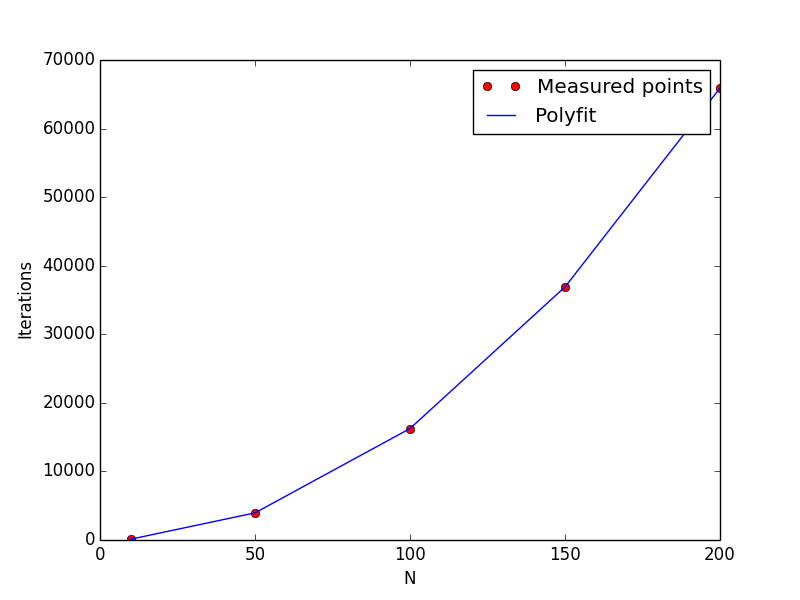
\includegraphics[scale=0.6]{Polyfit}
  \caption{Plot of the measured points and the result from the polyfit function. As we see the number of iterations goes as a second degree polynomial $1.6703N^2 - 4.5714N + 5.8511$}
\end{figure}

\subsection*{Ploting results}
\begin{figure}[H]
\centering
\subfloat[$\omega = 0.01$]{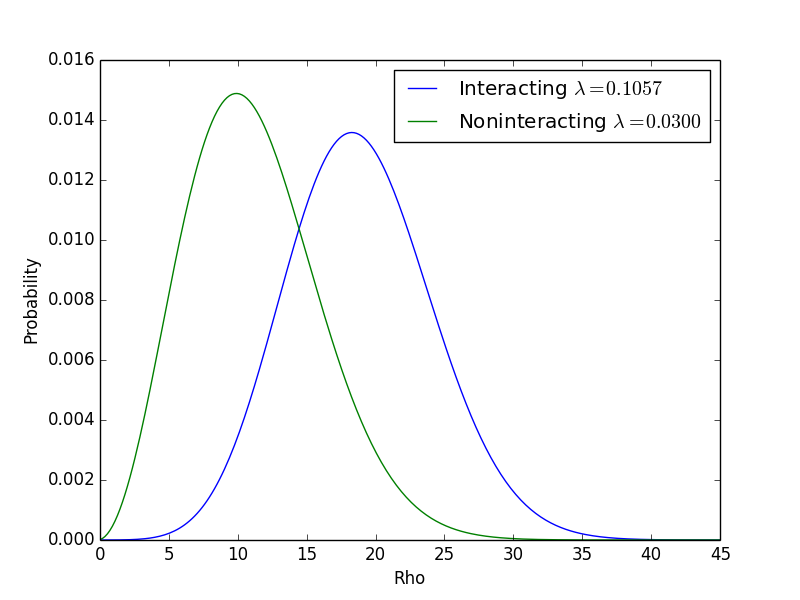
\includegraphics[width=0.5\textwidth]{ProbW001}}
\subfloat[$\omega = 0.5$]{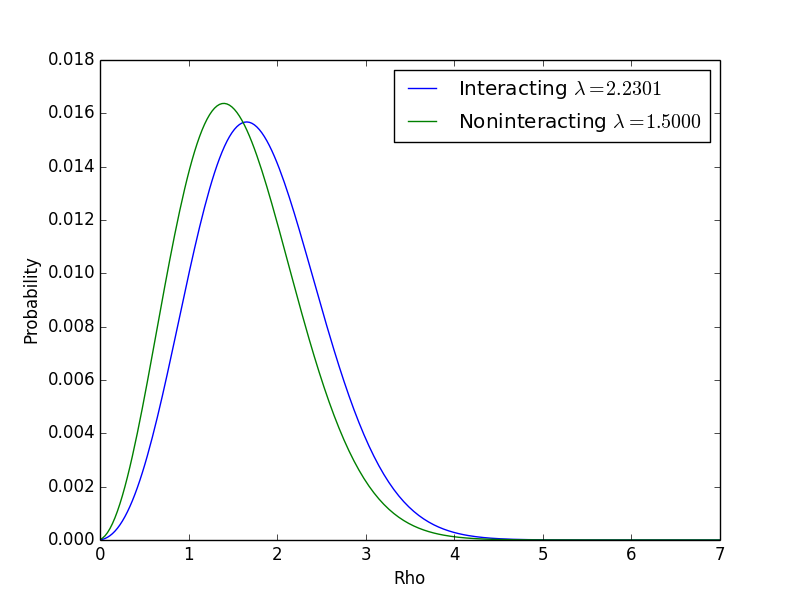
\includegraphics[width=0.5\textwidth]{ProbW05}}\\
\subfloat[$\omega = 1$]{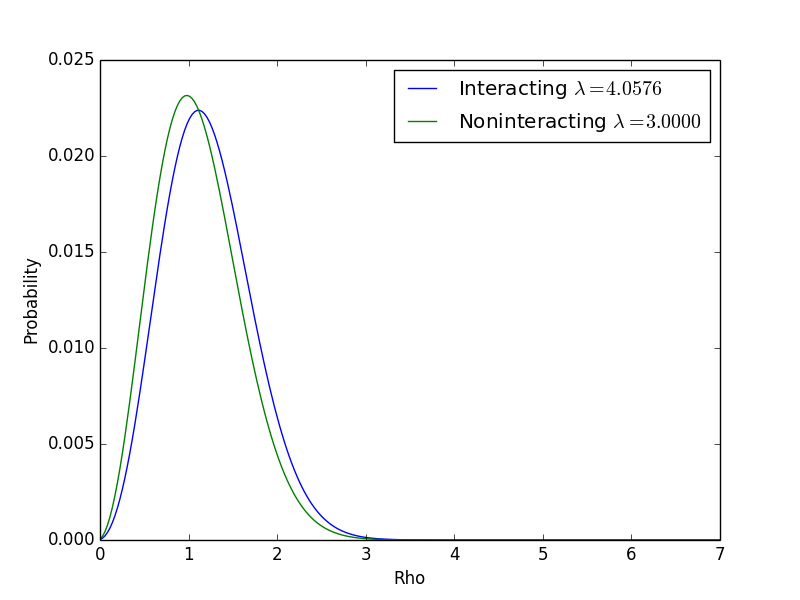
\includegraphics[width=0.5\textwidth]{ProbW1}}
\subfloat[$\omega = 5$]{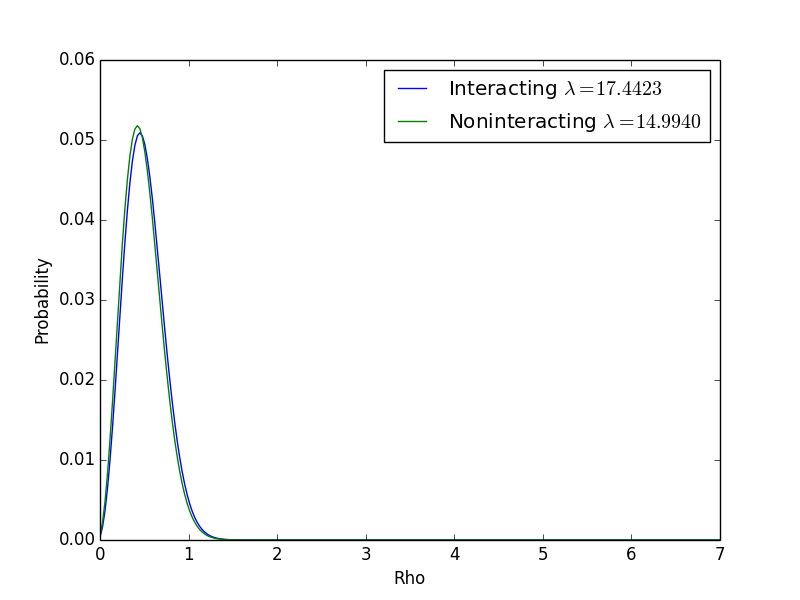
\includegraphics[width=0.5\textwidth]{ProbW5}}
\caption{The interacting and non-interacting probabilitydistributions between two electrons.}
\end{figure}

\begin{figure}[H]
\centering
\subfloat[$\omega = 0.01$]{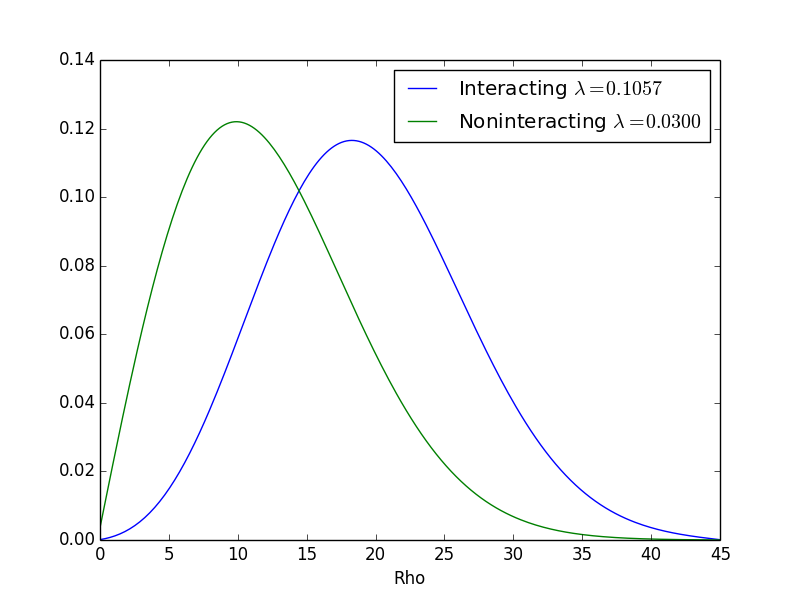
\includegraphics[width=0.5\textwidth]{W001}}
\subfloat[$\omega = 0.5$]{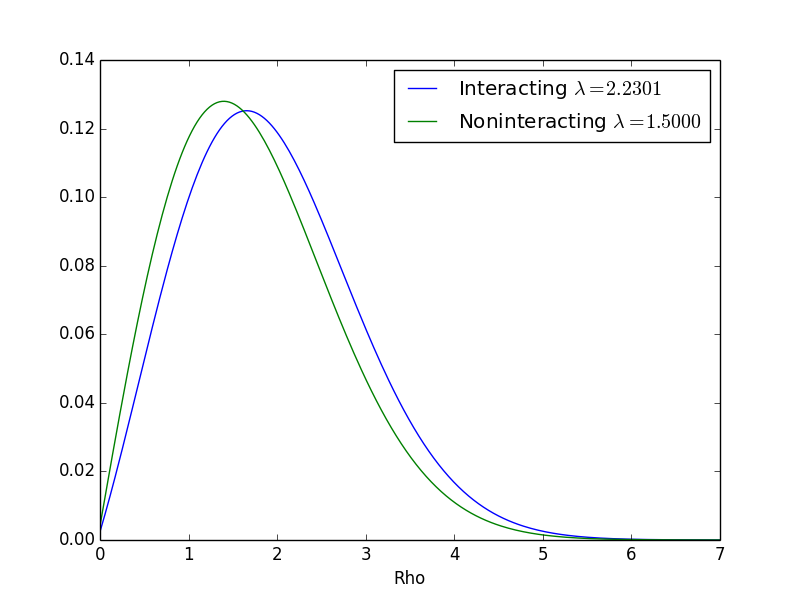
\includegraphics[width=0.5\textwidth]{W05}}\\
\subfloat[$\omega = 1$]{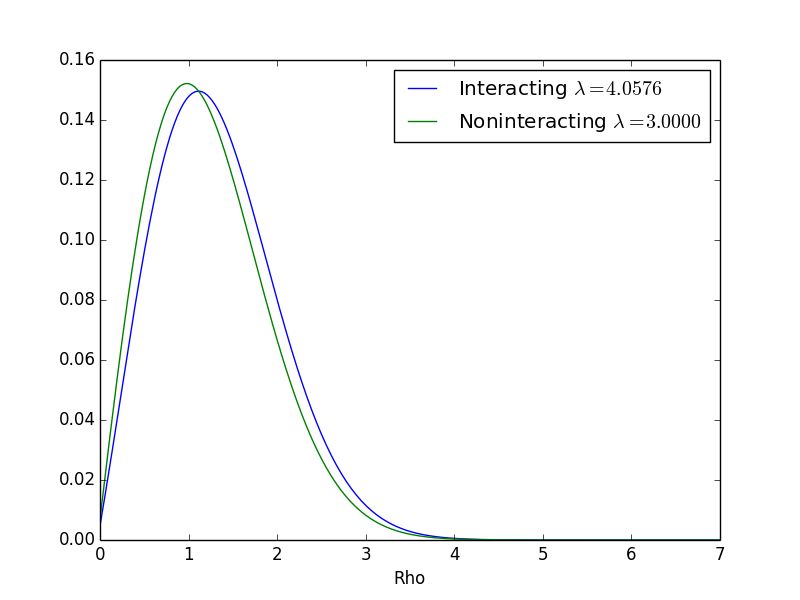
\includegraphics[width=0.5\textwidth]{W1}}
\subfloat[$\omega = 5$]{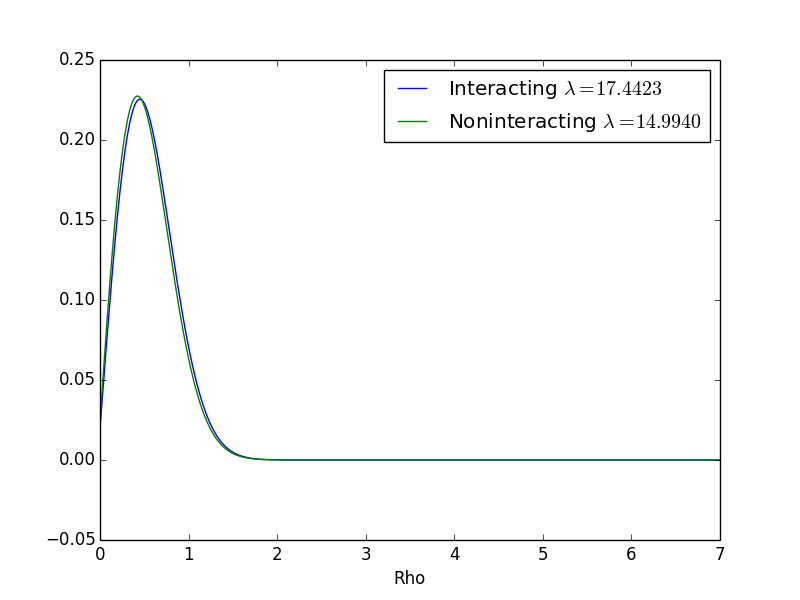
\includegraphics[width=0.5\textwidth]{W5}}
\caption{The interacting and non-interacting wavefunctions between two electrons.}
\end{figure}


As we can see in the plots, the distance between the electrons increases drastically when omega is small. For $omega = 0.01$, $\rho_{max}$ had to be increased to a minimum of 40 to contain the wavefunction. Increasing $\omega$ corresponds to increasing the part of the potential that is not repulsive, and we can see from the plot of $\omega = 5$ that the interacting and non-interacting case are almost equal. 

\section*{Conclusion}
The Jacobi method works very well as long as we do not work with very big matrices, because the number of iterations goes as a second degree function of the size of the matrix.\\
Using a suitable $\rho_{max}$ is important. If it is to small, it will not contain the entire wavefunction and the result for our energies will be wrong.\\
We have also seen that the strength of the potential in the wavefunction have a big impact on the probability of the relative distance between the electrons.



\end{document}
